\input{../header}

\begin{document}
%


%\onehalfspacing
\allowdisplaybreaks
%##################################################################
\section{PS\#10 - Separable differential equations - \red{Answer key} }

\everymath{\displaystyle}
\begin{enumerate}[leftmargin=0pt]

\item (\href{https://activecalculus.org/single/sec-7-4-separable.html#tjm}{AC 7.4 Exercise 6}) The mass of a radioactive sample decays at a rate that is proportional to its mass.
\begin{enumerate}
    \item Express this fact as a differential equation for the mass $M(t)$ using $k$ for the constant of proportionality.
    
    \begin{red}
    \[\frac{dM}{dt} = -kM\]
    (Setting it up this way, with a negative sign in front of $kM$, assumes that $k>0$ and tricks my brain into believing that this is indeed decay rather than growth.)
    \end{red}
    \item If the initial mass is $M_0$, find an expression for the mass $M(t)$.
    
    \begin{red}
    Separate and integrate. I'm going to use the usual trick of ``multiplying by $dt$'' which, we remember, is not exactly what's happening. I'm also going to use the usual trick of relabeling $e^C$ as a new constant to deal with the $\pm$ issue that would arise from dropping the absolute values on $M$.
    \begin{align*}
        \frac{dM}{dt} &= -kM \\
        \frac{1}{M}\ dM &= -k\ dt \\
        \int \frac{1}{M}\ dM &= \int -k\ dt \\
        \ln|M| &= -kt + C \\
        |M| &= e^{-kt+C} = e^{-kt} e^C \\
        M(t) &= Ce^{-kt} \\
        M_0 = M(0) &= Ce^0 = C \\
        M(t) &= M_0 e^{-kt}
    \end{align*}
    \end{red}
    \item The \textit{half-life} of the sample is the amount of time required for half of the mass to decay. Knowing that the half-life of Carbon-14 is 5730 years, find the value of $k$ for a sample of Carbon-14.
    
    \begin{red}
    From this information I know that $M(5730) = \frac12 M_0$. Therefore,
    \begin{align*}
        M_0e^{-k\cdot5730} &= \frac12 M_0 \\
        -k\cdot5730 &= \ln\left(\frac12\right) = -\ln(2) \\
        k &= \frac{\ln(2)}{5730}
    \end{align*}
    (So: in general, for a radioisotope with a half-life of $h$ years, the value of $k$ works out to be $\tfrac{\ln(2)}{h}$.)
    \end{red}
    \item How long does it take for a sample of Carbon-14 to be reduced to one-quarter its original mass?
    
    \begin{red}
    We want to solve $M(t) = \frac14 M_0$. Here comes some logarithm algebra:
    \begin{align*}
        M_0 e^{-kt} &= \frac14 M_0 \\
        -kt &= \ln\left(\frac14\right) = -\ln(4) \\
        t &= \frac{\ln(4)}{k} = \frac{\ln(4)}{\ln(2) / 5730} 
        = 5730\cdot \frac{\ln(4)}{\ln(2)} 
        = 5730\cdot \frac{\ln(2^2)}{\ln(2)} 
        = 5730\cdot \frac{2\ln(2)}{\ln(2)} 
        = 11460
    \end{align*}
    (a) logarithms are so cool; (b) this makes sense because to get to a quarter we should halve twice.
    \end{red}
    \item Carbon-14 naturally occurs in our environment; any living organism takes in Carbon-14 when it eats and breathes. Upon dying, however, the organism no longer takes in Carbon-14. Suppose that you find remnants of a pre-historic firepit. By analyzing the charred wood in the pit, you determine that the amount of Carbon-14 is only 30\% of the amount in living trees. Estimate the age of the firepit.
    
    \begin{red}
    So here we're going to solve $M(t) = 0.3M_0$:
    \begin{align*}
        M_0 e^{-kt} &= 0.3 M_0 \\
        -kt &= \ln(0.3) \\
        t &= \frac{\ln(0.3)}{-k} = \frac{\ln(0.3)}{-\ln(2)/5730} = 5730\cdot \frac{\ln(0.3)}{-\ln(2)} \approx 9952.81
    \end{align*}
    I'm going to conclude that the firepit is about ten thousand years old, give or take.
    \end{red}
\end{enumerate}

\item (\href{https://activecalculus.org/single/sec-7-4-separable.html#Zqv}{AC 7.4 Exercise 7}) Consider the initial value problem \[\frac{dy}{dt} = -\frac{t}{y}, \ y(0) = 8\]
\begin{enumerate}
    \item Find the solution of the initial value problem and sketch its graph.
    
    \begin{red}
    I'm going to use the usual trick of ``multiplying both sides by $dt$'' even though I know that's not really what's happening:
    \begin{align*}
        \frac{dy}{dt} &= -\frac{t}{y} \\
        y\ dy &= -t\ dt \\
        \int y\ dy &= \int -t\ dt \\
        \frac{y^2}{2} &= \frac{-t^2}{2} + C \\
        y^2 &= C - t^2
    \end{align*}
    I will pause here to note that $t^2 + y^2 = C$ is totally the equation of a circle, but that's not a function. Let's figure out the solution to this IVP; we're going to need to take a square root, and the initial value will help us decide about the $\pm$:
    \begin{align*}
        y(t) &= \pm\sqrt{C - t^2} \\
        8 = y(0) &= \pm \sqrt{C - 0^2}
    \end{align*}
    This means that we'll have to take the $+$ and that $C = 64$. Therefore, our solution is $y(t) = \sqrt{64 - t^2}$ -- the top half of a circle with radius 8.
    \end{red}
    \begin{center}
        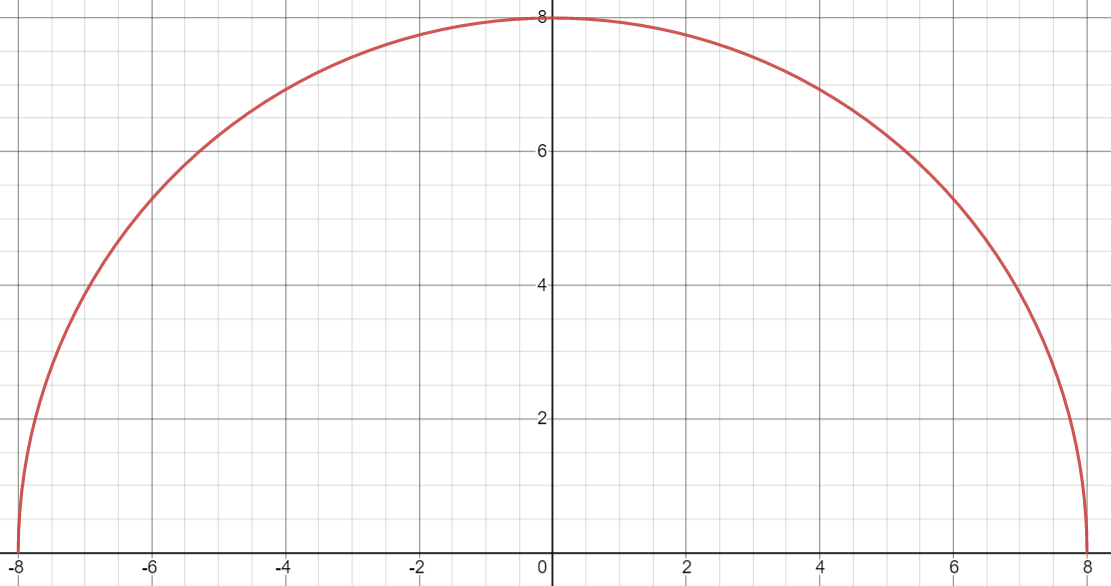
\includegraphics[width=0.7\textwidth]{../images/7.4.7.a.png}
    \end{center}
    \item For what values of $t$ is the solution defined?
    
    \begin{red}
    Since the square root of a negative number isn't defined (in the real numbers, anyway), $y(t)$ is only defined for $t$ in the range $-8\leq t \leq 8$.
    \end{red}
    \item What is the value of $y$ at the last time that the solution is defined?
    
    \begin{red}
    When $t=8$, $y(8) = \sqrt{64-8^2} = 0$.
    \end{red}
    \item By looking at the differential equation, explain why we should not expect to find solutions with the value of $y$ you noted in part (c). 
    
    \begin{red}
    Yeah, so that slope is wild: $\frac{dy}{dt} = -\frac{t}{y} = -\frac{8}{0}$. (Indeed, the tangent line to the side of the circle is vertical and thus has an undefined slope.)
    \end{red}
\end{enumerate}

\item (\href{https://activecalculus.org/single/sec-7-4-separable.html#FxE}{AC 7.4 Exercise 8}) Suppose that a cylindrical water tank with a hole in the bottom is filled with water. The water, of course, will leak out and the height of the water will decrease. Let $h(t)$ denote the height of the water. A physical principle called \textit{Torricelli's Law} implies that the height decreases at a rate proportional to the square root of the height.
\begin{enumerate}
    \item Express this fact using $k$ as the constant of proportionality.
    
    \begin{red}
    \[\frac{dh}{dt} = k\sqrt{h}\]
    \end{red}
    \item Suppose you have two tanks, one with $k = -1$ and another with $k=-10$. What physical differences would you expect to find?
    
    \begin{red}
    The tank with $k=-1$ is leaking much slower than the tank with $k=-10$. I'm going to say that the tank with $k=-10$ has a way smaller hole in the bottom.
    \end{red}
    \item Suppose you have a tank for which the height decreases at $20$ inches per minute when the water is filled to a depth of $100$ inches. Find the value of $k$.
    
    \begin{red}
    So this information is telling us that when $h = 100$, $\frac{dh}{dt} = -20$. Putting this information into our differential equation, we can figure out the value of $k$:
    \begin{align*}
        \frac{dh}{dt} &= k\sqrt{h} \\
        -20 &= k\sqrt{100} \\
        -20 &= 10k \\
        k &= -2
    \end{align*}
    \end{red}
    \item Solve the initial value problem for the tank in part (c), and graph the solution you determine.
    
    \begin{red}
    I'm going to use the usual trick of ``multiplying both sides by $dt$'' even though I know that's not really what's happening:
    \begin{align*}
        \frac{dh}{dt} &= -2\sqrt{h} \\
        \frac{1}{\sqrt{h}}\ dh &= -2\ dt \\
        \int h^{-1/2}\ dh &= \int -2\ dt \\
        \frac{h^{1/2}}{1/2} &= -2t + C \\
        \sqrt{h} &= -t + C \\
        h(t) &= (-t + C)^2 \\
    \intertext{To figure out the value of $C$, we're going to say that time $t=0$ is the moment when the tank was filled to a depth of $100$ inches. (That is, any other times we end up figuring out in this problem are measured in ``minutes after the tank had 100 inches of water in it.'')}
        100 = h(0) &= (-0 + C)^2 \\
        10 &= C \\
        h(t) &= (-t + 10)^2
    \end{align*}
    \end{red}
    \begin{center}
        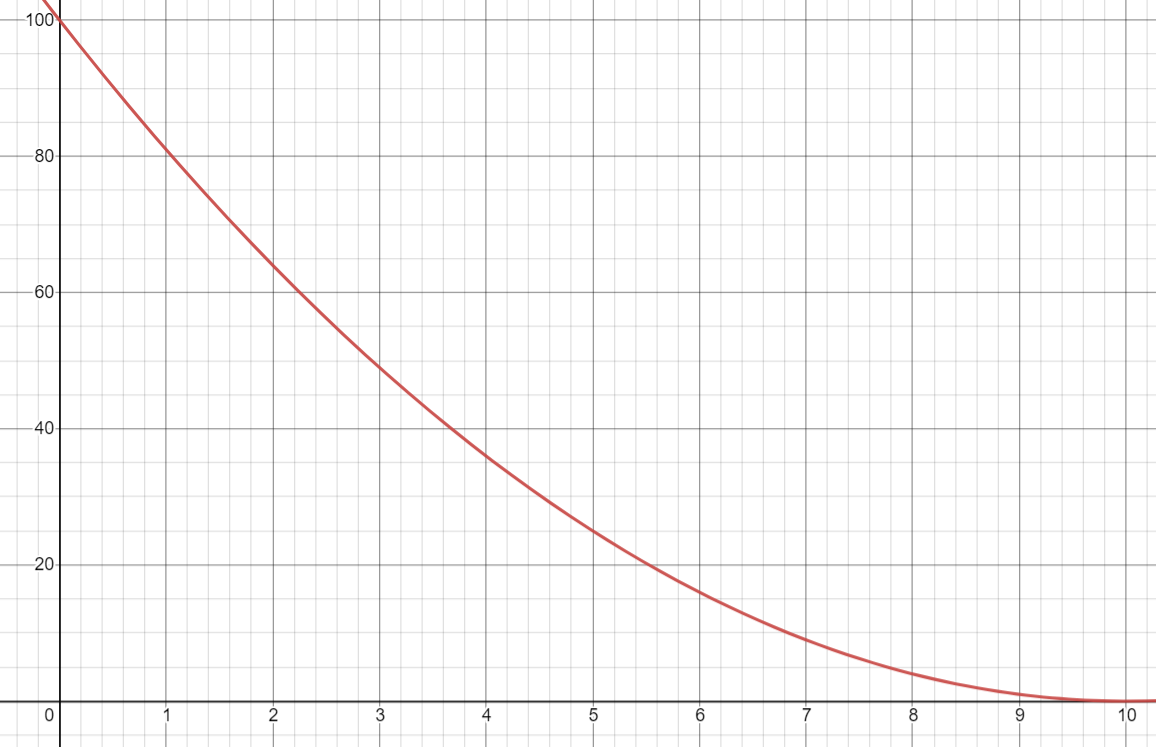
\includegraphics[width=0.7\textwidth]{../images/7.4.8.d.png}
    \end{center}
    \item How long does it take for the water to run out of the tank?
    
    \begin{red}
    $h(t) = 0$ when $t = 10$, so it takes 10 minutes (after the tank had 100 inches of water in it) for all the water to drain out.
    \end{red}
    \item Is the solution that you found valid for all time $t$? If so, explain how you know this. If not, explain why not.
    
    \begin{red}
    The solution predicts that the tank will start \textit{filling} again after $t=10$, which is clearly a silly prediction. So the solution certainly isn't valid beyond $t=10$.
    \end{red}
\end{enumerate}
\pagebreak

\item (\href{https://activecalculus.org/single/sec-7-4-separable.html#lEN}{AC 7.4 Exercise 9}) The \textit{Gompertz equation} is a model that is used to describe the growth of certain populations. Suppose that $P(t)$ is the population of some organism and that
\[\frac{dP}{dt} = -P\ln\left(\frac P3\right) = -P(\ln P - \ln 3) \]
\begin{enumerate}
    \item Sketch a slope field for $P(t)$ over the range $0\leq P \leq 6$.
    
    \begin{red}
    This also includes the solution curves at $P(0) = 1$ and $P(0) = 6$. Notice that I'm only including positive values for $t$.
    \end{red}
    \begin{center}
        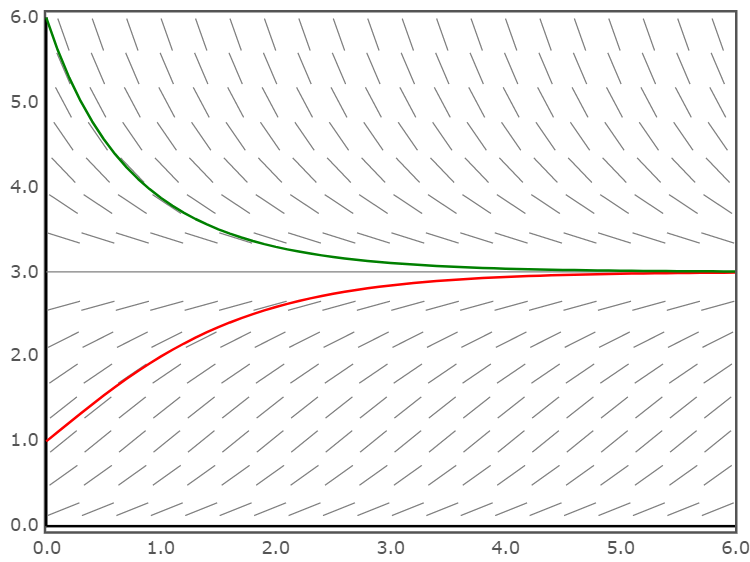
\includegraphics[width=0.5\textwidth]{../images/7.4.9.slopefield.png}
    \end{center}
    \item Identify any equilibrium solutions and determine whether they are stable or unstable.
    
    \begin{red}
    Looks like there's a stable equilibrium at $P = 3$, and indeed, when we set the differential equation equal to $0$ and solve for $P$, we get $-P\ln\left(\tfrac{P}{3}\right) = 0 $, so either $P=0$ or $\ln\left(\tfrac{P}{3}\right) = 0$.
    $P=0$ isn't a valid equilibrium solution because putting $P=0$ into the differential equation causes us to take $\ln(0)$, which doesn't exist, so we'll discard that one as extraneous. Therefore, we're left with $\ln\left(\tfrac{P}{3}\right) = 0$, so $\tfrac{P}{3} = 1$, so $P=3$.
    \end{red}
    \item Find the population $P(t)$ assuming  $P(0) = 1$ and sketch its graph. What happens to $P(t)$ after a very long time?
    
    \begin{red}
    I'm going to use the usual trick of ``multiplying both sides by $dt$'' even though I know that's not really what's happening. I'm also going to use the usual trick of relabeling $e^C$ as a new constant to deal with the $\pm$ issue that would arise from dropping the absolute values.
    \begin{align*}
        \frac{dP}{dt} &= -P(\ln P - \ln 3) \\
        \frac{1}{-P(\ln P - \ln 3)} \ dP &= 1\ dt \\
        \int \frac{1}{-P(\ln P - \ln 3)} \ dP &= \int 1\ dt = t + C\\
        \intertext{We'll make a $u$-substitution with $u = \ln P - \ln 3$. Then $du = \tfrac{1}{P}\ dP$.}
        \int\frac{1}{-u}\ du &= t + C \\
        -\ln|u| &= t + C \text{, so } \ln|u| = -t + C \\
        \ln|\ln P - \ln 3| &= -t + C \\
        |\ln P - \ln 3| &= e^{-t + C} = e^{-t} e^C \\
        \ln P - \ln 3 &= C e^{-t} \\
        \ln P &= C e^{-t} + \ln 3 \\
        P(t) &= e^{C e^{-t} + \ln 3} = e^{C e^{-t}} e^{\ln 3} = 3 e^{C e^{-t}}
    \end{align*}
    (Type $P(t) = 3 e^{C e^{-t}}$ into Desmos and play with the slider that comes up for $C$!)
    
    At this point we can use our initial condition to find the value of $C$. If $\displaystyle 1 = P(0) = 3 e^{C e^{-0}} = 3 e^C$, then \\ $C = \ln(1/3) = -\ln 3$.
    Therefore, our solution is $P(t) = 3 e^{-\ln(3) e^{-t}}$. It appears that the long-run behavior of this solution is indeed to tend toward our stable equilibrium at $P=3$.
    \end{red}
    \begin{center}
        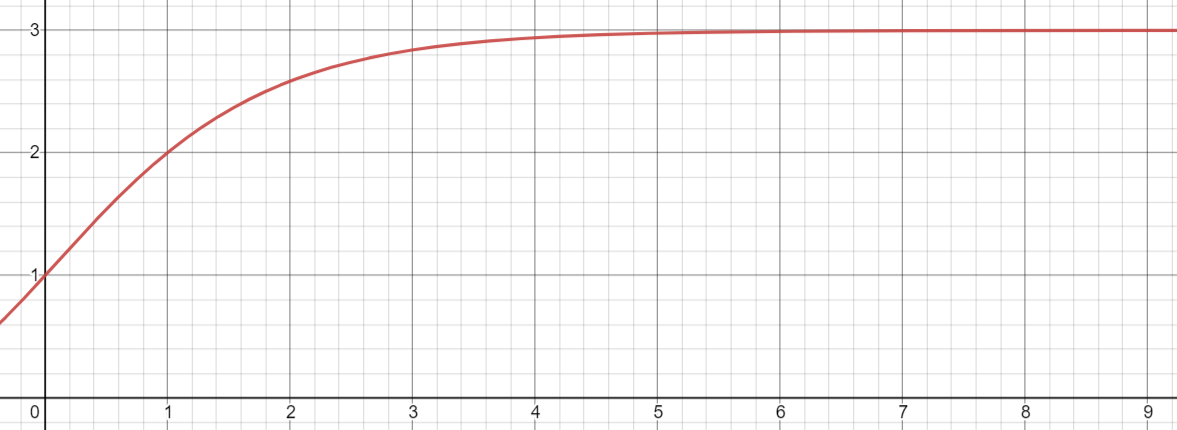
\includegraphics[width=0.7\textwidth]{../images/7.4.9.c.png}
    \end{center}
    \item Find the population $P(t)$ assuming $P(0) = 6$ and sketch its graph. What happens to $P(t)$ after a very long time?
    
    \begin{red}
    If $\displaystyle 6 = P(0) = 3 e^{C e^{-0}} = 3 e^C$, then $C = \ln(2)$.
    Therefore, our solution is $P(t) = 3 e^{\ln(2) e^{-t}}$. It appears that the long-run behavior of this solution is indeed to tend toward our stable equilibrium at $P=3$.
    \end{red}
    \begin{center}
        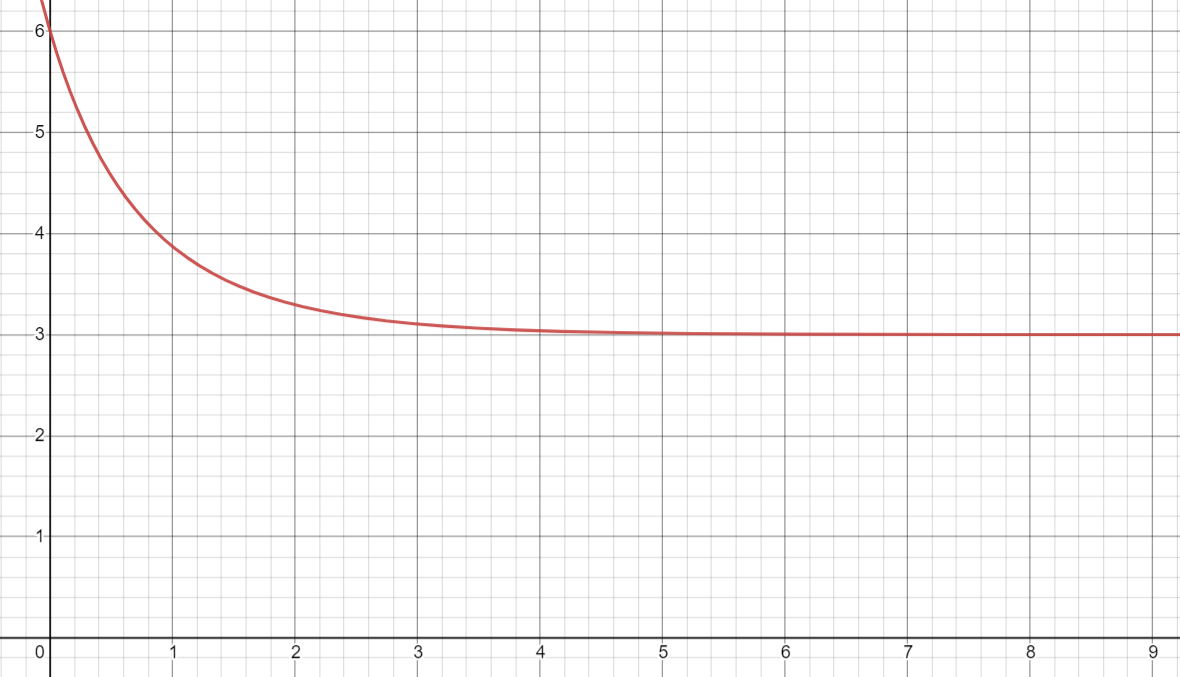
\includegraphics[width=0.7\textwidth]{../images/7.4.9.d.png}
    \end{center}
    \item Verify that the long-term behavior of your solutions agrees with what you predicted by looking at the slope field.
    
    \begin{red}
    Yep, this looks right: both of our solutions are indeed trending toward the stable equilibrium at $P=3$.
    \end{red}
\end{enumerate}

\end{enumerate}
\end{document}